This guide provides an introduction to using Haizea in simulation mode. Even if you intend to use Haizea in combination with another system, such as OpenNebula, you may still find this guide useful to familiarize yourself with the Haizea configuration file and command-line interface. This guide assumes that you've downloaded and installed Haizea. Also, make sure you've read the What is Haizea? page before following this guide.

\section{The \texttt{haizea} command}

The main command in the Haizea system is, unsurprisingly, the haizea command. Running this command starts up the Haizea lease manager, which is then ready to receive and schedule lease requests. When running Haizea in simulation mode, lease requests are read from a tracefile, a text file containing a list of lease requests. Based on these requests, the simulator produces a schedule for those leases, which you will be able to follow through the logging messages printed by Haizea. At the end of the simulation, Haizea also saves a fair amount of raw data and statistics to disk which can be used to produce reports and graphs (a module to do this for you is in the works).

When not running in simulation, Haizea runs as a daemon that can accept requests (e.g., through a command-line interface) and sends out enactment commands ("start VM", "stop VM", etc.) to the appropriate enactment module. For example, when running OpenNebula with Haizea as a scheduling backend, Haizea is in charge of processing the requests received by OpenNebula, coming up with a schedule, and then instructing OpenNebula on when VMs should be start/stop/suspend/resume on what physical nodes. A document describing how to use Haizea with OpenNebula will be available soon.

But, anyway, back to how to run Haizea in simulation. The first thing we need to do is to write a configuration file specifying simulation options (e.g., the characteristics of the simulated cluster) and scheduling options.

\section{The configuration file}

A sample configuration file is provided with Haizea and is located in /usr/share/haizea/etc/sample.conf (or \$HOME/share/haizea/etc/sample.conf if you installed Haizea in your home directory). For this guide, you may want to make a copy of this file and use that instead (so you can preserve the original sample file). If you look at the contents of the file, you will see that it also includes documentation on every option. For now, take a look at the following three options:

\begin{wideshellverbatim}
[simulation]
starttime: 2006-11-25 13:00:00
nodes: 4
resources: CPU,1;Mem,1024;Net (in),100;Net (out),100;Disk,20000
\end{wideshellverbatim}

These options are used to describe the characteristics of our simulated cluster. In particular, we're using a 4-node cluster, each node with 1 CPU, 1024 MB of memory, 20GB of disk space, and 100Mbps of inbound/outbound network bandwidth. In this document, we will represent this cluster over time like this:

\begin{center}
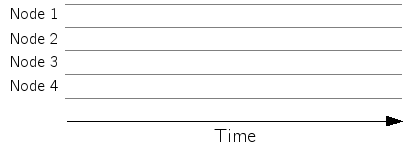
\includegraphics{images/quickstart_leasegraph1.png}
\end{center}

For example, the following figure shows a lease scheduled on Node 1 from 13:00 to 14:00:

\begin{center}
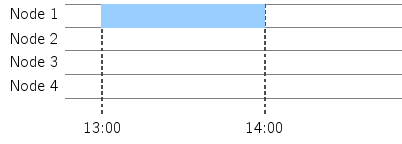
\includegraphics{images/quickstart_leasegraph2.png}
\end{center}

The starttime option is used to specify the time at which the simulated clock should start. As you will see, the configuration file has an abundance of other options. We will explain some of them in this document.

\section{The tracefile}

As mentioned earlier, the simulator will read trace requests from a tracefile. The location of this tracefile is specified in the configuration file, in the \texttt{[tracefile]} section:

\begin{wideshellverbatim}
[tracefile]
tracefile: /usr/share/haizea/traces/sample.lwf 
\end{wideshellverbatim}

The default value is a sample tracefile included with Haizea. If you copy the file to a different location, make sure to update the tracefile option accordingly. The format of this file is LWF (Lease Workload Format), which is particular to Haizea. The sample file includes documentation on the file format, and several sample workloads. For now, we will focus on the first workload, "PREEMPT":

\begin{wideshellverbatim}
# 0   -1   3600 3600 1 1 1024 0 foobar.img 1024
# 900 1800 1800 1800 4 1 1024 0 foobar.img 1024
\end{wideshellverbatim}

For now, don't worry about parsing the trace format in detail. The above represents two lease requests:

\begin{itemize}
\item The first line is a request for a best-effort lease, requested at time 0 (right at the start of the simulation), requiring 1 hour (3600 seconds), and only one node.
\item The second line is an advance reservation (AR) lease, requested 15 minutes into the simulation (900 seconds), starting 30 minutes into the simulation (1800 seconds), requiring 30 minutes (1800 seconds), and all four nodes in the cluster. Since the start time of the simulation is set to 13:00, this means the lease request is received at 13:15, and that the lease must run from 13:30 to 14:00.
\end{itemize}

Both leases require 1 CPU per node, 1024 MB of memory, a disk image called "foobar.img" (which uses up 1024MB of disk space). The \# characters are used to comment out the lease requests. Do not change this for now.

\section{Running the simulator}

Now that we have a configuration file and a tracefile, we can run the simulator. As shown in the installation guide, you can run Haizea with the sample configuration file like this:

\begin{shellverbatim}
haizea -c /usr/share/haizea/etc/sample.conf 
\end{shellverbatim}

Which results in the following output:

\begin{wideshellverbatim}
[2006-11-25 13:00:00.00] TFILE   Loading tracefile /usr/share/haizea/traces/sample.lwf
[2006-11-25 13:00:00.00] TFILE   Loaded workload with 0 requests (0 best-effort + 0 AR)
[2006-11-25 13:00:00.00] RM      Starting resource manager
[2006-11-25 13:00:00.00] CLOCK   Starting simulated clock
[2006-11-25 13:00:00.00] CLOCK   Stopping simulated clock
[2006-11-25 13:00:00.00] RM      Stopping resource manager
[2006-11-25 13:00:00.00] RM        Completed best-effort leases: 0
[2006-11-25 13:00:00.00] RM        Accepted AR leases: 0
[2006-11-25 13:00:00.00] RM        Rejected AR leases: 0
\end{wideshellverbatim}

Now that you've seen the tracefile, you can see why the simulator starts up and immediately stops: all the lease requests in the tracefile are commented out, and there's nothing to schedule. Go ahead and uncomment only the first lease request and run Haizea again. You should now see the following:

\begin{wideshellverbatim}
[2006-11-25 13:00:00.00] TFILE   Loading tracefile /usr/share/haizea/traces/sample.lwf
[2006-11-25 13:00:00.00] TFILE   Loaded workload with 1 requests (1 best-effort + 0 AR)
[2006-11-25 13:00:00.00] RM      Starting resource manager
[2006-11-25 13:00:00.00] CLOCK   Starting simulated clock
[2006-11-25 13:00:00.00] SCHED   Received (and queueing) best-effort lease request #1, 
                                 1 nodes for 01:00:00.00.
[2006-11-25 13:00:00.00] SCHED   Next request in the queue is lease 1. 
                                 Attempting to schedule...
[2006-11-25 13:00:00.00] SLOT    Lease #1 has been scheduled on nodes [1] 
                                 from 2006-11-25 13:00:00.00 
                                   to 2006-11-25 14:00:00.00
[2006-11-25 13:00:00.00] SCHED   Started VMs for lease 1 on nodes [1]
[2006-11-25 14:00:00.00] SCHED   Stopped VMs for lease 1 on nodes [1]
[2006-11-25 14:00:00.00] CLOCK   Stopping simulated clock
[2006-11-25 14:00:00.00] RM      Stopping resource manager
[2006-11-25 14:00:00.00] RM        Completed best-effort leases: 1
[2006-11-25 14:00:00.00] RM        Accepted AR leases: 0
[2006-11-25 14:00:00.00] RM        Rejected AR leases: 0
\end{wideshellverbatim}

The above corresponds to the following schedule:

\begin{center}
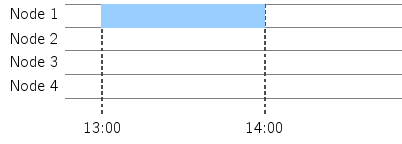
\includegraphics{images/quickstart_leasegraph2.png}
\end{center}

A best-effort request is received at 13:00 and, since the cluster is empty, it is scheduled immediately. Notice how the VMs for the lease start at 13:00 and stop at 14:00. For now, we're assuming that the disk images are predeployed on the physical nodes (we will modify this option in the next section).

So, what would happen if we also added the AR lease? Since it requires all the cluster resources from 13:30 to 14:00, the best-effort lease will be unable to run in that time interval. Since the leases are implemented as VMs, Haizea will still schedule the best-effort lease to start at 13:00, but will suspend it before the AR lease starts, and will resume it one the AR lease has finished. In effect, we want the schedule to look like this:

\begin{center}
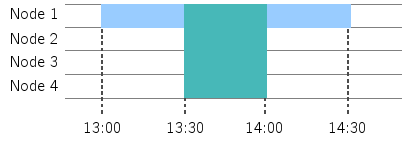
\includegraphics{images/quickstart_leasegraph3.png}
\end{center}

Uncomment the AR lease request, and run Haizea again. You should now see the following (for clarity, log messages pertaining to the best-effort lease are highlighted in green, and those pertaining to the AR lease are highlighted in brown):

\begin{wideshellverbatim}
[2006-11-25 13:00:00.00] TRACE   Loading tracefile /usr/share/haizea/traces/sample.lwf
[2006-11-25 13:00:00.00] TRACE   Loaded workload with 2 requests (1 best-effort + 1 AR)
[2006-11-25 13:00:00.00] RM      Starting resource manager
[2006-11-25 13:00:00.00] CLOCK   Starting simulated clock
[2006-11-25 13:00:00.00] SCHED   Received (and queueing) best-effort lease request #1, 
                                 1 nodes for 01:00:00.00.
[2006-11-25 13:00:00.00] SCHED   Next request in the queue is lease 1. 
                                 Attempting to schedule...
[2006-11-25 13:00:00.00] SLOT    Lease #1 has been scheduled on nodes [1] 
                                 from 2006-11-25 13:00:00.00 
                                   to 2006-11-25 14:00:00.00
[2006-11-25 13:00:00.00] SCHED   Started VMs for lease 1 on nodes [1]

[2006-11-25 13:15:00.00] SCHED   Received AR lease request #2, 4 nodes 
                                 from 2006-11-25 13:30:00.00 
                                   to 2006-11-25 14:00:00.00.
[2006-11-25 13:15:00.00] SCHED   Must preempt leases [1] to make room for AR lease #2
[2006-11-25 13:15:00.00] SCHED   Preempting lease #1...
[2006-11-25 13:15:00.00] SCHED   ... lease #1 will be suspended 
                                     at 2006-11-25 13:30:00.00.
[2006-11-25 13:15:00.00] SCHED   AR lease request #2 has been accepted.

[2006-11-25 13:29:39.00] SCHED   Stopped VMs for lease 1 on nodes [1]
[2006-11-25 13:29:39.00] SCHED   Suspending lease 1...

[2006-11-25 13:30:00.00] SCHED   Lease 1 suspended.
[2006-11-25 13:30:00.00] SCHED   Started VMs for lease 2 on nodes [2, 3, 4, 1]
[2006-11-25 13:30:00.00] SCHED   Next request in the queue is lease 1. 
                                 Attempting to schedule...
[2006-11-25 13:30:00.00] SLOT    Lease #1 has been scheduled on nodes [1] 
                                 from 2006-11-25 14:00:21.00 (resuming) 
                                   to 2006-11-25 14:30:42.00

[2006-11-25 14:00:00.00] SCHED   Stopped VMs for lease 2 on nodes [2, 3, 4, 1]
[2006-11-25 14:00:00.00] SCHED   Resuming lease 1...

[2006-11-25 14:00:21.00] SCHED   Resumed lease 1
[2006-11-25 14:00:21.00] SCHED   Started VMs for lease 1 on nodes [1]

[2006-11-25 14:30:42.00] SCHED   Stopped VMs for lease 1 on nodes [1]
[2006-11-25 14:30:42.00] CLOCK   Stopping simulated clock
[2006-11-25 14:30:42.00] RM      Stopping resource manager
[2006-11-25 14:30:42.00] RM        Completed best-effort leases: 1
[2006-11-25 14:30:42.00] RM        Accepted AR leases: 1
[2006-11-25 14:30:42.00] RM        Rejected AR leases: 0
\end{wideshellverbatim}

Notice how the above corresponds to the previous figure. In particular, notice the following:

\begin{itemize}
 \item  When the AR lease request is received, Haizea looks at the schedule and determines that the only way to schedule the AR lease is to preempt the best-effort lease. However, instead of canceling that lease, it will just reschedule it so it is suspended right before the AR lease start. Note that Haizea will always try to minimize the number of preemption (in this case, we're forcing the situation for demonstration purposes) by assigning the AR lease to resources that are available without preempting other leases.
 \item Shortly before the AR lease starts, the best-effort lease is suspended (the time required to do this is estimated by Haizea based on an option in the configuration file). When the AR lease ends at 14:00, Haizea begins resuming the suspended best-effort lease.
\end{itemize}

\section{The scheduling options}

Haizea has several scheduling options that control how Haizea selects resources and schedules leases. For example, the above example assumed that leases can be suspended (which they generally always can be when running as virtual machines). What would happen if this were not possible? You can modify the suspension option in the [scheduling] section to find out:

[scheduling]
...

suspension: none

...

Rerun Haizea. Now, when the AR lease arrives at 13:15, the scheduler will realize it has to preempt the best-effort lease to make room for the AR lease, but will no longer be able to suspend it. The only option is to cancel the best-effort lease and resubmit it to the queue:

\begin{wideshellverbatim}
[2006-11-25 13:15:00.00] SCHED   Preempting lease #1...
[2006-11-25 13:15:00.00] SCHED   ... lease #1 has been cancelled and requeued
                                     (cannot be suspended)
\end{wideshellverbatim}

Now, the best-effort lease can only be scheduled after the AR lease, at 14:00:

\begin{wideshellverbatim}
[2006-11-25 13:15:00.00] SLOT    Lease #1 has been scheduled on nodes [1] 
                                 from 2006-11-25 14:00:00.00 
                                   to 2006-11-25 15:00:00.00
\end{wideshellverbatim}

So, the schedule would end up looking like this:

\begin{center}
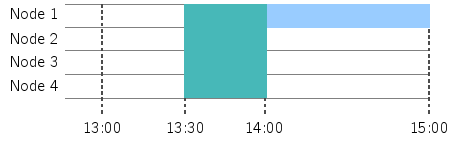
\includegraphics{images/quickstart_leasegraph4.png}
\end{center}

Notice how, although suspending a lease is a disruptive activity which can delay the completion time of a best-effort request, it is still much better than completely canceling a request and waiting for enough resources to accommodate the entire (uninterrupted) duration of the lease.

Another scheduling option you can modify is whether Haizea should transfer the VM's disk image from an image repository before the lease can start. You can do this by modifying the lease-deployment option:

\begin{wideshellverbatim}
[general]
...
lease-deployment: imagetransfer
...
\end{wideshellverbatim}

If you look at the bottom of the sample configuration file, you will find a section called \texttt{[deploy-imagetransfer]} with all the image transfer options.

Rerun Haizea again. You should get a schedule similar to the previous one, but with some extra messages indicating that image transfers are taking place:

[2006-11-25 13:00:00.00] SCHED   Starting image transfer for lease 1
[2006-11-25 13:01:22.00] SCHED   Completed image transfer for lease 1

As you can see, the best-effort lease can no longer start right at 13:00, since an image transfer has to take place before the starting time. The same is true of the AR lease, but notice how Haizea schedules the image transfer in such a way that the AR lease can still start at 13:30 as planned (instead of delaying the starting time until 13:31:22).

There are several other options you can modify in the [scheduling] section, such as what backfilling algorithm to use, whether to allow lease migration or not, etc. See the description of these option in the sample configuration file for more details.
Other things you can do with Haizea

At this point, you can run simple simulations with Haizea. However, there is a lot more that you can do with Haizea:

\begin{itemize}
\item Run on real hardware: First and foremost, everything you just saw above in simulation can be done on real hardware. This is accomplished by using Haizea with the OpenNebula virtual infrastructure manager. So, if you have a Xen or KVM cluster, you can just install OpenNebula and Haizea to enable your users to request VM-based leases on your cluster.
\item Run complex simulations: The above shows only two leases on a 4-node cluster during a span of roughly 2 hours. Boring. Haizea can handle more complex simulations, and also provides the necessary tools for you to easily run multiple simulations with different profiles. For example, in the Haizea paper Combining Batch Execution and Leasing Using Virtual Machines we simulated running 72 30-day workloads in six different configurations, or 36 years of lease scheduling. To set up this kind of simulations, take a look at the Running Multiple Simulation Experiments with Haizea document.
\item Produce reports and graphs: The above examples relied on you reading the Haizea log messages, which is ok for a simple simulation, but no fun when you're scheduling thousands of leases. Haizea saves a fair amount of raw data to disk with scheduling metrics, utilization information, etc. which can be used to generate reports and graphs. We are in the process of producing tools that will allow you to easily analyse that data and create graphs.
\end{itemize}